\section{MVC}
\subsection{Moduł wejść}
W projekcie wykorzystane zostały zserializowane dane w formacie binarnym „*.dat”. To oznacza, że program obsługuje tylko pliki z dołączonego do projektu folderu SampleData. W wypadku, kiedy użytkownik chciałby skorzystać z innych danych istnieją dwa rozwiązania:

\begin{itemize}
\item Można wykorzystać skrypt dołączony do projektu (\ref{sec:skrypt}). Aby go uruchomić konieczne jest wcześniejsze pobranie z bazy Physionet oprogramowania ATM.  Ta opcja jest dostępna dla użytkowników,  którzy  chcą pobrać dane zawierające dwa sygnały.
\item Można pobrać oprogramowanie ATM , pobrać odpowiednie pliki i skonwertować je do formatu *.txt . Ta opcja odpowiednia jest dla plików zawierających sygnały z 12 elektrod i wykorzystywana jest tylko w module VCG\_T\_LOOP .
\end{itemize}

Taki sposób wczytywania danych jest optymalny pod względem szybkości działania programu, zdecydowanie utrudnia jednak korzystanie z innego rodzaju danych niż dostarczone. 

\subsection{Struktura aplikacji.}
Istotnym z punktu widzenia rozwoju aplikacji zagadnieniem są współzależności modułów, czyli określenie kolejności wywoływania modułów. Ogólny schemat przedstawiony jest poniżej (\ref{fig:zaleznosci}). Moduły wywoływane są rekurencyjnie w takim sensie, że w przypadku braku potrzebnych danych wywołany zostanie moduł wyżej. W efekcie każdy moduł można uruchomić jednym kliknięciem. W przypadku, w którym odpowiednie dane zostały już przetworzone, wywoływany moduł nie zażąda wywołania modułu nadrzędnego. To oznacza, że po każdej zmianie parametrów wszystkie kolejne moduły należy wywoływać ręcznie, w odpowiedniej kolejności. 

\begin{figure}[H]
\centering
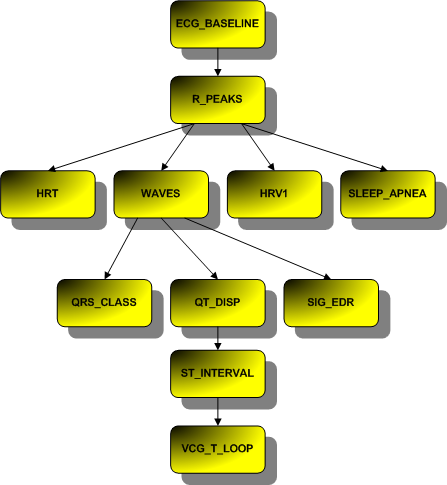
\includegraphics[scale=0.7]{MVC/img/EKG}
\label{fig:zaleznosci}
\caption{Schemat zależności modułow aplikacji}
\end{figure}

Poza modułami w projekcie występują następujące klasy:
\begin{itemize}
\item „appcontroller” czyli klasa zarządzająca całym programem.
\item „airecgmain”, wraz z klasami pomocniczymi, czyli klasa obsługująca GUI.
\item „ecgdata”, wraz z klasami pomocniczymi, czyli klasa przechowująca dane.
\item „ecgentry”, wraz z klasami pomocniczymi, czyli klasa wczytująca dane binarne z pliku.
\end{itemize}

Całość projektu jest tworzona według wzorca Model-View-Controller. Oznacza to, że te trzy części są od siebie wyraźnie rozdzielone. Zarówno widoki (prezentacja wyników), jak i kontroler (interakcja z użytkownikiem) realizowana jest w całości przez GUI. Model (wszystkie obliczenia) wykonywane są w odpowiednich modułach, które nie muszą być dołączane do projektu. Zarządzanie tymi elementami realizowane (czyli silnik aplikacji) realizowane jest przez klasę „appcontroller”. Spełnienie ogólnego wzorca MVC w praktyce oznacza, że klasa appcontroller jest jedyną klasą, która może wymagać modyfikacji po zmodyfikowaniu któregokolwiek innego elementu programu.

\subsection{Logi}

Poza normalnym działaniem aplikacja oferuje również logowanie przebiegu ostatniego wywołania aplikacji z użyciem pakietu QsLog. Do logu zapisywane są najważniejsze zdarzenia i błędy. Raportowany jest także czas wykonania wpisu, co pozwala na oszacowanie szybkości działania poszczególnych modułów, w zależności od wybranych w GUI parametrów. Przykładowy log przedstawiony jest poniżej. Logger można wykorzystać także do pomiaru czasów wykonywania poszczególnych elementów programu. Przykładowe czasy, uzyskane dla sygnału złożonego z 649999 próbek, zamieszczono w tabeli ref!!!!.

\begin{table}
|ECG_BASELINE | 0.538 |
\end{table}

\begin{minipage}{\textwidth}
\begin{verbatim}
 INFO 2014-01-29T22:23:34.965 Program started 
 INFO 2014-01-29T22:24:01.591 Stworzono obiekt typu ecgdata dla pacjenta  "107" . 
 INFO 2014-01-29T22:24:01.756 "649999"  Samples loaded 
 INFO 2014-01-29T22:24:01.841 Reset procedure started: 
 INFO 2014-01-29T22:24:01.841 MVC/ Sleep Apnea deleted 
 INFO 2014-01-29T22:24:01.841 All removed. 
 INFO 2014-01-29T22:24:07.936 Start AtrialFibr 
 INFO 2014-01-29T22:24:07.936 Waves started. 
 INFO 2014-01-29T22:24:07.936 RPeaks stared. 
 INFO 2014-01-29T22:24:07.937 Ecg baseline started. 
 INFO 2014-01-29T22:24:07.937 BASELINE/ Using butterworth filter with coefficiets  "Baseline wander removal (Fs: 360Hz) - [HP, Order: 10, -3db: 0.5Hz]" 
 INFO 2014-01-29T22:24:07.937 MVC/  "V1"  signal will be processed. 
 INFO 2014-01-29T22:24:08.477 Ecg baseline done. 
 INFO 2014-01-29T22:24:08.542 RPeaks/ using Hilbert 
 INFO 2014-01-29T22:24:23.031 RPeaks done. 
 INFO 2014-01-29T22:24:37.838 Waves/ calculated  "2114"  QRS_onset points. 
 INFO 2014-01-29T22:24:37.838 Waves/ calculated  "2114"  QRS_end points. 
 INFO 2014-01-29T22:24:37.838 Waves/ calculated  "1029"  PWaveStart points. 
 INFO 2014-01-29T22:24:37.839 Waves/ calculated  "908"  PWaveEnd points. 
 INFO 2014-01-29T22:24:37.902 GUI/  ecgFrames.Count... "908" 
 INFO 2014-01-29T22:24:37.927 Waves done. 
TRACE 2014-01-29T22:24:37.931 Atrial_FIBR/ calculated parameters: 
 Atrial_FIBR/ PWaveOccurenceRatio:  "0.208941" 
 Atrial_FIBR/ RRIntDivergence:  "0.0319016" 
 Atrial_FIBR/ RRIntEntropy:  "0.219118" 
 INFO 2014-01-29T22:24:37.931 AtrialFibr done 
\end{verbatim}
\end{minipage}

\subsection{Skrypt przetwarzający dane.}
\label{sec:skrypt}

\begin{minipage}{\textwidth}
\begin{verbatim}
REM written by mickl , AGH UST
CLS
@ECHO OFF
ECHO Hello ,
REM ECHO PhysioNet availabl  indexes : 100 -124 , 200-234
REM SET /p index=Please insert record index
SET /a index=100
: loop
IF %index%==125 GOTO assign
IF %index%==235 GOTO quit

ECHO Downloading samples , record #%index%
rdsamp -r mitdb/%index% > %index%a.txt
ECHO Succesfully saved %index%a.txt
ECHO Serializing data
serializer.exe %index%a.txt %index%.dat
DEL %index%a.txt
ECHO Removing 101a.txt
ECHO Downloading annotations, record #%index%
rdann -r mitdb/%index% -a atr > %index%c.txt
ECHO Succesfully saved %index%c.txt
ECHO Downloading notes , record #%index%
wfdbdesc mitdb/%index% >%index%d.txt
ECHO Succesfully saved %index%d.txt

SET /a index=%index%+1
GOTO loop

: assign
SET /a index=200
GOTO loop

: quit
ECHO All records converted
\end{verbatim}
\end{minipage}